% Copyright 2024 Kieran W Harvie. All rights reserved.

\section{Clebsch–Gordan Coefficients}
Moving from classical mechanics where a system with two subsystems $V_1$ and $V_2$ is identified with $V_1\oplus V_2$ to quantum mechanic where it's instead identified with $V_1\otimes V_2$ brings many interesting changes.
A notable change is how angular momentum begins to add in a counterintuitive way which lead to a lot of systemizations:
"It's a vector!", "No it's a rotating cone!", "No the cones have to be set up a certain way!".
Well I'm going to do some revision and work my way back up to the Clebsch–Gordan coefficients.
\\

Let $\hat{j}$ be the angular momentum operator and $\hat{j}_z$ the operator for the projection of angular momentum on the $z$-axis, and like wise for $\hat{j}_x$ and $\hat{j}_y$.
Physically these that these operators satisfy the following commuting relations:
\[[\hat{j}_x,\hat{j}_y]=i\hbar\hat{j}_z,\quad
[\hat{j}_y,\hat{j}_z]=i\hbar\hat{j}_x,\quad
[\hat{j}_z,\hat{j}_x]=i\hbar\hat{j}_y\]
Which can be shorten to:
\[[\hat{j}_k,\hat{j}_l]=i\hbar\varepsilon_{klm}\hat{j}_m\]
Where $\varepsilon_{jkm}$ is the standard Levi-Civita symbol where we identify $x$ with $1$, $y$ with $2$, $z$ with $3$.
\\

The first problem with the transition is already clear,
these operators don't commute!
To work around this problem we instead consider the operator $\hat{j}^2$
\[\hat{j}^2 = \hat{j}_x^2+\hat{j}_y^2+\hat{j}_z^2\]
This operator does commute with the projection onto the axis:
\begin{equation*}
\begin{aligned}
	[\hat{j}^2,\hat{j}_z] =& (\hat{j}_x^2j_z-j_z\hat{j}_x^2)+(\hat{j}_y^2\hat{j}_z-\hat{j}_z\hat{j}_y^2)+(\hat{j}_z^2\hat{j}_z-\hat{j}_z\hat{j}_z^2) \\
	=& \hat{j}_x[\hat{j}_x,j_z]+[\hat{j}_x,j_z]\hat{j}_x+\hat{j}_y[\hat{j}_y,\hat{j}_z]+[\hat{j}_y,\hat{j}_z]\hat{j}_y \\
	=& i\hbar(-\hat{j}_x\hat{j}_y-\hat{j}_y\hat{j}_x+\hat{j}_y\hat{j}_x+\hat{j}_x\hat{j}_y) \\
	=& \hat{0}\\
\end{aligned}
\end{equation*}
This means we can find a common eigenbasis of $\hat{j}_z$ and $\hat{j}^2$\footnote{
	And likewise for $\hat{j}_x$ and $\hat{j}_y$ (but only one at a time) however $z$ is the conventional axis.
	Also I can't shake the feeling that I'm missing some point when getting a common eigenbasis from commuting hermitian operators.}.
We label these states $\ket{j,m}$ and,
for application reasons,
the relationship between the eigenvalues and labels aren't as expected.
Instead of using the eigenvalue as the label they are related by:
\begin{equation*}
\begin{aligned}
	\hat{j}^2\ket{j,m} =& \hbar^2 j(j+1)\ket{j,m},\quad j\in\left\{0,\frac{1}{2},1,\frac{3}{2},\cdots\right\}&\\
	\hat{j}_z\ket{j,m} =& \hbar m\ket{j,m}\,\quad m\in\left\{-j,-j+1,\cdots,j-1,j\right\}&\\
\end{aligned}
\end{equation*}

Note that an immediate result from $\hat{j}$ and $\hat{j}_k$ being hermitian is that their eigenvalues are real,
meaning we only have to assume $m\in\mathbb{Z}$ since:
\[\begin{aligned}
	j(j+1) =& \frac{1}{\hbar^2}\bra{j,m}\hat{j}^2\ket{j,m}\\
	=&\frac{1}{\hbar^2}\bra{j,m}\hat{j}^2_x\ket{j,m}+\frac{1}{\hbar^2}\bra{j,m}\hat{j}^2_y\ket{j,m}+\frac{1}{\hbar^2}\bra{j,m}\hat{j}^2_z\ket{j,m}\\
	\geq& \frac{1}{\hbar^2}\bra{j,m}\hat{j}_z^2\ket{j,m}\\
	=& m^2
\end{aligned}\]

\subsection{Total Angular Momentum}
The total angular momentum $\hat{J}$ on $V_1\otimes V_2$ is defined as expected:
\[\hat{J} = \hat{j_1}\otimes\hat{I}_2+\hat{I}_1\otimes\hat{j_2}\]
Observe that the left element of the tensor product always has to be from $V_1$ and carries a $1$ subscript,
and like wise for right and $2$.
This is annoying (even the identity elements need them),
so will be omitted.
Since we will be in the same tensor product space remember which space each element has to be from an mentally append the subscript.
\\

In this convention the total angular momentum operator would be written as:
\[\hat{J} = \hat{j}\otimes\hat{I}+\hat{I}\otimes\hat{j}\]
And the projection onto the $k$th axis as
\[\hat{J}_k = \hat{j}_k\otimes\hat{I}+\hat{I}\otimes\hat{j}_k\]

\subsubsection{Commutator Identities}
We will use the following two commutator identities:
\[[A\otimes B\,,\,C\otimes D] = (AC)\otimes(BD)-(BD)\otimes(AC)\]
\[[A+B,C+D] = [A,C]+[A,D]+[B,C]+[B,D]\]
And the following two sub cases of the first:
\[[A\otimes \hat{I}\,,\,C\otimes \hat{I}] = [A,C]\otimes\hat{I}\]
\[[A\otimes \hat{I}\,,\,\hat{I}\otimes D] =\hat{0}\]
While these identities can be directly algebraically verified they are worth clearly saying up front.

\subsubsection{Commuting Problems}
Unfortunately $\hat{J_k}$ follows the same commuting identities of $\hat{j_k}$,
preventing common eigenstates:
\begin{equation*}
\begin{aligned}
	[\hat{J}_k\,,\,\hat{J}_l] =& [\hat{j}_k\otimes\hat{I}+\hat{I}\otimes\hat{j}_k\,,\,\hat{j}_l\otimes\hat{I}+\hat{I}\otimes\hat{j}_l] \\
	=&[\hat{j}_k\otimes\hat{I}\,,\,\hat{j}_l\otimes\hat{I}]+[\hat{j}_k\otimes\hat{I}\,,\,\hat{I}\otimes\hat{j}_l] \\
	&+[\hat{I}\otimes\hat{j}_k\,,\,\hat{j}_l\otimes\hat{I}]+[\hat{I}\otimes\hat{j}_k\,,\,\hat{I}\otimes\hat{j}_l] \\
	=& [\hat{j}_k\,,\,\hat{j}_l]\otimes \hat{I}+\hat{I}\otimes[\hat{j}_k\,,\,\hat{j}_l]\\
	=& i\hbar\varepsilon_{klm}(\hat{j}_m\otimes\hat{I}+\hat{I}\otimes\hat{j}_m)\\
	=& i\hbar\varepsilon_{klm}\hat{J}_m\\
\end{aligned}
\end{equation*}
But this isn't such a big deal,
since we also have:
\[[\hat{J}^2,\hat{J}_z]=\hat{0}\]
However the use of $\hat{J}^2$ comes with its own problem in an awkward cross term: 
\[\hat{J}^2 = \hat{j}^2\otimes\hat{I}+\hat{I}\otimes\hat{j}^2+2\hat{j}\otimes\hat{j}\]

\subsubsection{Bases}
These results give us two bases for $V_1\otimes V_2$.
First is the natural basis from its definition as a tensor product:
\[\ket{m_1,j_1}\otimes\ket{m_2,j_2} = \ket{m_1,m_2,j_1,j_2}\]
With the natural interpretation of the subsystem $V_1$ being $\ket{m_1,j_1}$ and $V_2$ being in $\ket{m_2,j_2}$.
Second is the common eigenbasis of the commuting hermitian operators $\hat{J}^2$ and $\hat{J}_z$ defined by:
\begin{equation*}
\begin{aligned}
	\hat{J}^2\ket{J,M} =& \hbar^2 J(J+1)\ket{J,M}\\
	\hat{J}_z\ket{J,M} =& \hbar M\ket{J,M}\\
\end{aligned}
\end{equation*}
With the natural interpretation of the angular momentum and projected angular momentum of the supersystem.
We can convert between the two,
i.e. given the total angular momentum calculate the superposition subsystems or vise-versa,
is done in the normal way:
\[\ket{J,M} = \sum_{m_1,m_2,j_1,j_2}\ket{m_1,m_2,j_1,j_2}\braket{m_1,m_2,j_1,j_2}{J,M}\]
Note that despite the bounds being absent the use of a sum is justified by $\ket{m_1,m_2,j_1,j_2}$ being a base,
hence any state is in the span.
\\

But there's still a lot of them can we know in advance in any are $0$?
Well consider the following manipulation:
\[\begin{aligned}
	&\sum_{m_1,m_2,j_1,j_2}\hbar(m_1+m_2)\ket{m_1,m_2,j_1,j_2}\braket{m_1,m_2,j_1,j_2}{J,M}\\
	=&\sum_{m_1,m_2,j_1,j_2}(\hat{j}_z\otimes\hat{I}+\hat{I}\otimes\hat{j}_z)\ket{m_1,m_2,j_1,j_2}\braket{m_1,m_2,j_1,j_2}{J,M}\\
	=&\sum_{m_1,m_2,j_1,j_2}\hat{J}_z\ket{m_1,m_2,j_1,j_2}\braket{m_1,m_2,j_1,j_2}{J,M}\\
	=&\hat{J}_z\sum_{m_1,m_2,j_1,j_2}\ket{m_1,m_2,j_1,j_2}\braket{m_1,m_2,j_1,j_2}{J,M}\\
	=&\hat{J}_z\ket{J,M}\\
	=&\hbar M\ket{J,M}\\
	=&\hbar M\sum_{m_1,m_2,j_1,j_2}\ket{m_1,m_2,j_1,j_2}\braket{m_1,m_2,j_1,j_2}{J,M}\\
\end{aligned}\]
Taking the first expression away from the final gives:
\[
	0=\sum_{m_1,m_2,j_1,j_2}\hbar(M-(m_1+m_2))\ket{m_1,m_2,j_1,j_2}\braket{m_1,m_2,j_1,j_2}{J,M}\\
\]
Hence the coefficients must be $0$ unless $M=m_1+m_2$.

\subsection{Clebsch–Gordan Coefficients}
Consider the case where we fix $j_1$ and $j_2$ of the subsystems along side the $J$ and $M$ of the supersystem.
This is a common application when the subsystems are elementary particles with fixed $j_1$ and $j_2$ and the supersystem is in a state with fixed $J$ and $M$ due to externalities. 
Instead of considering the whole of $V_1\otimes V_2$ instead just consider the subspace:
\[\spn\{\ket{m_1,j_1}\mid\{|m_1|\leq j_1\}\}\otimes\spn\{\ket{m_2,j_2}\mid\{|m_2|\leq j_2\}\}\]
After proving closure everything we proved about $V_1\otimes V_2$ applies here,
prefixing $[j_1,j_2]$ to the kets to denote the subspace,
or dropping when the meaning is clear.
We can use these results to express the supersystem as a superposition of different $m_1$ and $m_2$.
\[\ket{[j_1,j_2],J,M} = \sum_{k=-j_1}^{j_1}\ket{k,M-k,j_1,j_2}\braket{k,M-k,j_1,j_2}{[j_1,j_2]J,M}\]
(Note, alternative parametrizations of this sum are common and available)
These coefficients $\braket{m_1,m_2,j_1,j_2}{J,M}$ are the Clebsch–Gordan coefficients and can be looked up in readily available and iconically shaped tables.

\subsection{Rotating Cones}
In the beginning I talked about interpreting quantum angular momentum as rotating cones,
what did I mean by this?
Well consider the set of points in $\mathbb{R}^3$ with a known distance to the origin and known $Z$ component.
We get a circle centered on the $Z$ axis at that known hight.
The analogy to quantum angular momentum is obvious:
\begin{center}
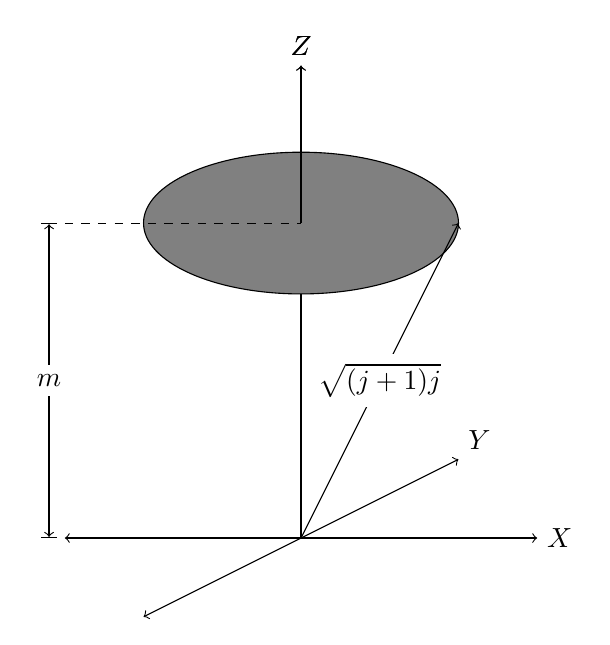
\begin{tikzpicture}
	\draw[<->] (-3,0)--(3,0) node[right]{$X$};
	\draw[->] (0,0)--(0,6) node[above]{$Z$};
	\draw[<->] (-2,-1)--(2,1) node[above right]{$Y$};
	\draw[fill = gray] (0,4) circle[x radius = 2, y radius = 0.9];
	\draw[->] (0,4)--(0,6) node[above]{$Z$};

	\draw[dashed] (-3,4)--(0,4);
	\draw[|<->|] (-3.2,0)--  (-3.2,4) node[midway,fill=white]{$m$};

	\draw[->] (0,0)--(2,4) node[midway,fill=white]{$\sqrt{(j+1)j}$} ;
\end{tikzpicture}
\end{center}
But how do we add momentum this way?
Well if we consider the most simple case of adding a one of these disks to to itself.
We simply take one point on the edge of the disk and scale up accordingly:
\begin{center}
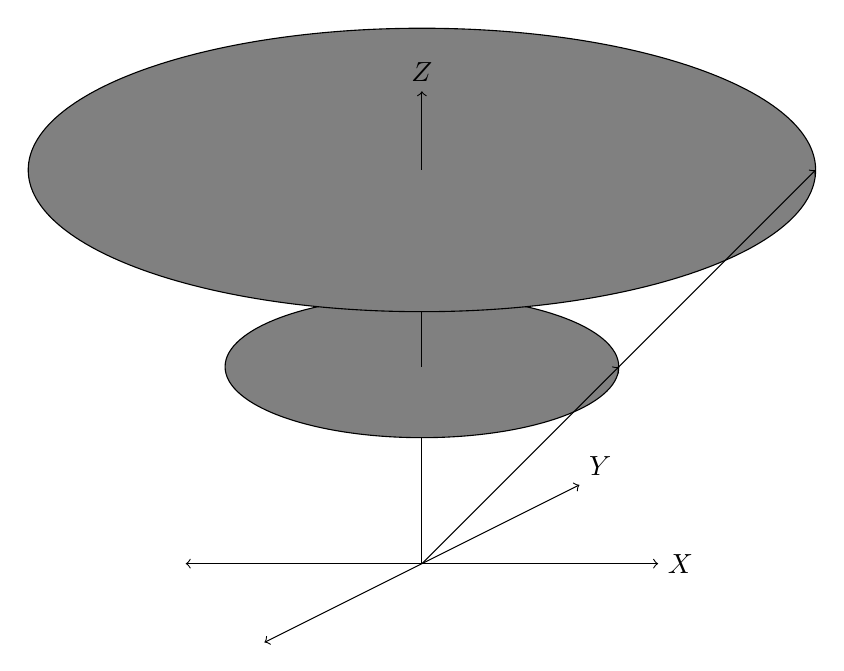
\begin{tikzpicture}
	\draw[<->] (-3,0)--(3,0) node[right]{$X$};
	\draw[<->] (-2,-1)--(2,1) node[above right]{$Y$};
	\draw (0,0)--(0,2.5);
	\draw[fill = gray] (0,2.5) circle[x radius = 2.5, y radius = 0.9];
	\draw (0,2.5)--(0,5);
	\draw[fill = gray] (0,5) circle[x radius = 5, y radius = 1.8];
	\draw[->] (0,5)--(0,6) node[above]{$Z$};

	\draw[->] (0,0)--(2.5,2.5);
	\draw[->] (2.5,2.5)--(5,5);
\end{tikzpicture}
\end{center}
This corresponds to the following equation:
\[\ket{\left[\frac{1}{2},\frac{1}{2}\right],1,1}=\frac{1}{\sqrt{2}}\left(\ket{\frac{1}{2},\frac{1}{2}}+\ket{\frac{1}{2},\frac{1}{2}}\right)\]
But this idea isn't complete because we need to incorporate relative phase of the basis vectors into the picture.
For example we have could be in phase:
\begin{center}
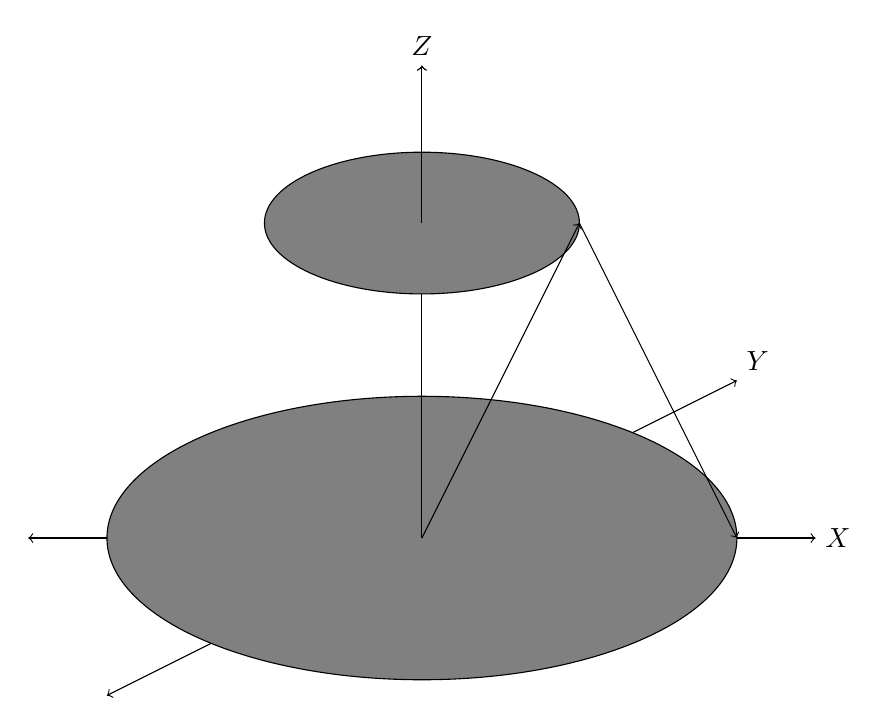
\begin{tikzpicture}
	\draw[<->] (-5,0)--(5,0) node[right]{$X$};
	\draw[<->] (-4,-2)--(4,2) node[above right]{$Y$};
	\draw[fill = gray] (0,0) circle[x radius = 4, y radius = 1.8];
	\draw[->] (0,0)--(0,6);
	\draw[fill = gray] (0,4) circle[x radius = 2, y radius = 0.9];
	\draw[->] (0,4)--(0,6) node[above]{$Z$};

	\draw[->] (0,0)--(2,4);
	\draw[->] (2,4)--(4,0);
\end{tikzpicture}
\end{center}
\[\ket{1,0}=\frac{1}{\sqrt{2}}\left(\ket{\frac{1}{2},-\frac{1}{2}}+\ket{-\frac{1}{2},\frac{1}{2}}\right)\]
As well as in opposite phase:
\begin{center}
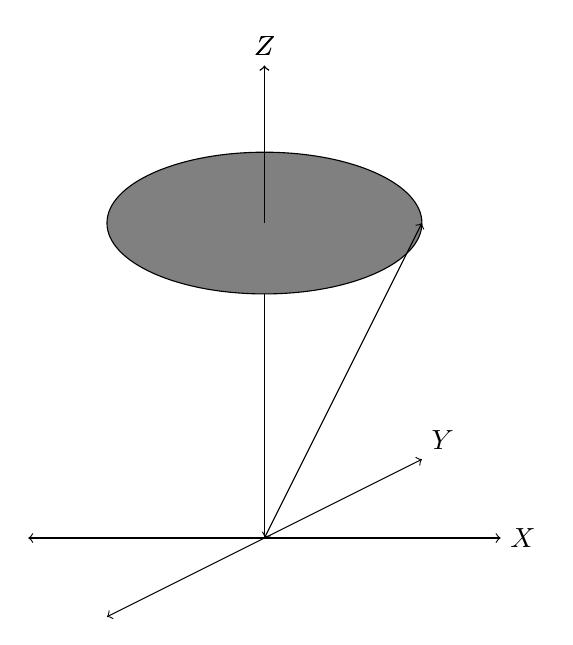
\begin{tikzpicture}
	\draw[<->] (-3,0)--(3,0) node[right]{$X$};
	\draw[->] (0,0)--(0,6) node[above]{$Z$};
	\draw[<->] (-2,-1)--(2,1) node[above right]{$Y$};
	\draw[fill = gray] (0,4) circle[x radius = 2, y radius = 0.9];
	\draw[->] (0,4)--(0,6) node[above]{$Z$};

	\draw[<->] (0,0)--(2,4);
\end{tikzpicture}
\end{center}
\[\ket{0,0}=\frac{1}{\sqrt{2}}\left(\ket{\frac{1}{2},-\frac{1}{2}}-\ket{-\frac{1}{2},\frac{1}{2}}\right)\]
As suggested by the picture the relative phase of the basis vectors is the relative phase of the $\mathbb{R}^3$ vectors as they rotate around.
In the first example the two basis vectors are in phase so both vectors start at $0$ degrees and rotate together.
While in the second example the two basis vectors are in opposite phase so one starts at $0$ degrees and the other at $180$ meaning as they rotate they cancel out.
\\

This is what's meant by "Rotating cones set up a certain way".
First you convert vectors into cones using the initial geometry analogy.
Then you scale them by the basis vectors' coefficients relative magnitude and rotate them by their relative phase.
Finally you rotate the vectors at the same angular velocity and see which disk is traced out.
\\

(Note the reason they are disks instead of cones is because it's surprisingly difficult to draw cones in tikz.
The reader is invited to use their imagination to fill in the missing sides.)

\subsection{Conclusion}
The previous section concludes the revision I needed and I'm getting kind of tired of thinking about Clebsch–Gordan theory.
However the topic is rich and I can see myself coming back later and appending to this section,
bellow is a wish-list of explorations on my return:
\begin{itemize}
	\item Actually calculating some Clebsch–Gordan coefficients.
		I normally just look them up confident someone has done them correctly.
	\item Talk about the total angular momentum raising and lowering operators:
		\[\hat{J}_\pm = \hat{j}_\pm\otimes I + I\otimes\hat{j}_\pm\]
	\item Talk about Lie Algebras.
		Both how they apply to the communicator section in general and how the calculations used here are the basis of a representation of the SU(2) Lie Algebra.
	\item There relationship between the coefficients and spherical harmonics.
\end{itemize}
